\chapter{Heat Engines and Machines}\label{ch:b1:heat-engines}

A car engine, a power station, a \omterm{def:b1:heat-engines:machine}{refrigerator} and a \omterm{def:b1:heat-engines:machine}{heat pump} are the
same object seen from four sides: a fluid taken round a cycle, in
contact by turns with a hot source and a cold one, exchanging heat with
both and work with a shaft. The first law bookkeeps the energy; the
second law, through the entropy balance over one cycle, sets the limit
that no cleverness can beat --- Carnot's theorem, the most consequential
inequality of engineering. This chapter derives that limit, computes
the ideal cycle and the real ones that approach it (Otto, Diesel,
Stirling), turns the machine round to make cold and to heat houses,
and shows how the created entropy of a real machine is paid for, joule
by joule, in \omterm{thm:b1:heat-engines:lostwork}{lost work}.

\section{Cyclic machines and the two laws}

\begin{definition}[Thermodynamic machine]\label{def:b1:heat-engines:machine}
\index{heat engine}\index{refrigerator}\index{heat pump}\index{thermostat}
A \emph{thermodynamic machine} is a \omterm{def:b1:newton-dynamics:conservation}{closed system} (the working fluid)
taken round a \emph{cycle}, so that it returns periodically to the same
state, while exchanging work $W$ with the outside and heat $Q_i$ with
sources at temperatures $T_i$ --- \emph{thermostats}, whose temperature
the exchange does not change. A \emph{ditherm} machine uses two
thermostats, the hot source at $T_h$ and the cold source at $T_c < T_h$.
It is an \emph{engine} if it delivers work ($W < 0$), a
\emph{refrigerator} if it is driven ($W > 0$) to take heat from the cold
source, a \emph{heat pump} if it is driven to give heat to the hot one.
All quantities are reckoned over one cycle, algebraically, as received
by the fluid.
\end{definition}

\begin{theorem}[The two laws over a cycle; Clausius inequality]\label{thm:b1:heat-engines:clausius}
\index{Clausius inequality}
Over one cycle of a ditherm machine,
\[
W + Q_h + Q_c = 0 , \qquad
\frac{Q_h}{T_h} + \frac{Q_c}{T_c} = -S_{\mathrm{created}} \leq 0 ,
\]
with equality in the second relation if and only if the cycle is
reversible. More generally, for any number of \omterm{def:b1:heat-engines:machine}{thermostats},
$\sum_i Q_i/T_i \leq 0$ (\emph{Clausius inequality}).
\end{theorem}

\begin{proof}
$U$ and $S$ are state functions, so $\Delta U = 0$ and $\Delta S = 0$ over
a cycle. The first law gives $0 = W + Q_h + Q_c$; the entropy balance
(\cref{thm:b1:second-law-entropy:secondlaw}) gives $0 = S_{\mathrm{exch}} +
S_{\mathrm{created}}$ with $S_{\mathrm{exch}} = \sum Q_i/T_i$ because each
\omterm{def:b1:heat-engines:machine}{thermostat} exchanges at its own fixed temperature
(\cref{prop:b1:second-law-entropy:thermostat}).
\end{proof}

\begin{corollary}[Kelvin again]\label{cor:b1:heat-engines:kelvin}
A \emph{monotherm} machine ($Q_c = 0$) has $Q_h \leq 0$, hence $W \geq 0$:
no cycle can convert the heat of a single source into work. A ship
cannot sail by cooling the sea --- an engine needs a cold source to
reject heat to, and the second law says how much it must reject.
\end{corollary}

\begin{omfigure}
\begin{tikzpicture}[font=\small, x=1cm, y=1cm, >=Stealth]
  % engine
  \begin{scope}
    \draw[fill=omThm!15, draw=omThm, thick] (-1.6,3.0) rectangle (1.6,3.7) node[midway] {hot source $T_h$};
    \draw[fill=omDef!15, draw=omDef, thick] (-1.6,-0.7) rectangle (1.6,0) node[midway] {cold source $T_c$};
    \draw[thick, rounded corners, fill=omProp!10] (-0.9,1.0) rectangle (0.9,2.0) node[midway] {engine};
    \draw[->, omThm, very thick] (0,3.0) -- (0,2.0) node[midway, right] {$Q_h > 0$};
    \draw[->, omDef, very thick] (0,1.0) -- (0,0) node[midway, right] {$Q_c < 0$};
    \draw[->, omProp, very thick] (0.9,1.5) -- (2.3,1.5) node[midway, above] {$W < 0$};
    \node[font=\footnotesize] at (0,-1.1) {$\eta = -W/Q_h$};
  \end{scope}
  % refrigerator / heat pump
  \begin{scope}[xshift=6.4cm]
    \draw[fill=omThm!15, draw=omThm, thick] (-1.6,3.0) rectangle (1.6,3.7) node[midway] {hot source $T_h$};
    \draw[fill=omDef!15, draw=omDef, thick] (-1.6,-0.7) rectangle (1.6,0) node[midway] {cold source $T_c$};
    \draw[thick, rounded corners, fill=omProp!10] (-1.1,1.0) rectangle (1.1,2.0) node[midway, align=center, font=\footnotesize] {refrigerator\\ or heat pump};
    \draw[->, omThm, very thick] (0,2.0) -- (0,3.0) node[midway, right] {$Q_h < 0$};
    \draw[->, omDef, very thick] (0,0) -- (0,1.0) node[midway, right] {$Q_c > 0$};
    \draw[->, omProp, very thick] (-2.5,1.5) -- (-1.1,1.5) node[midway, above] {$W > 0$};
    \node[font=\footnotesize] at (0,-1.1) {$e_f = Q_c/W$, \quad $e_p = -Q_h/W$};
  \end{scope}
\end{tikzpicture}

{\small The two ways round a ditherm cycle. Left: the engine takes heat
from the hot source, rejects part of it to the cold one and delivers the
difference as work. Right: the same machine driven backward pumps heat
from cold to hot; it is a \omterm{def:b1:heat-engines:machine}{refrigerator} if one wants $Q_c$, a \omterm{def:b1:heat-engines:machine}{heat pump}
if one wants $|Q_h|$.}
\end{omfigure}

\section{Carnot's theorem}

\begin{definition}[Efficiency and coefficients of performance]\label{def:b1:heat-engines:efficiency}
\index{efficiency!of a heat engine}\index{coefficient of performance}
The \emph{efficiency} of an engine is the work delivered per unit heat
taken from the hot source, $\eta = -W/Q_h$; the
\emph{coefficient of performance} (COP) of a \omterm{def:b1:heat-engines:machine}{refrigerator} is the cold
produced per unit work, $e_f = Q_c/W$; that of a \omterm{def:b1:heat-engines:machine}{heat pump} is the heat
delivered per unit work, $e_p = -Q_h/W$. Each is the ratio ``what one
wants'' over ``what one pays''; an efficiency is at most~1, a COP can
exceed~1.
\end{definition}

\begin{theorem}[Carnot]\label{thm:b1:heat-engines:carnot}
\index{Carnot's theorem}\index{Carnot efficiency}
Between \omterm{def:b1:heat-engines:machine}{thermostats} $T_h > T_c$,
\[
\eta \leq \eta_C = 1 - \frac{T_c}{T_h}, \qquad
e_f \leq \frac{T_c}{T_h - T_c}, \qquad
e_p \leq \frac{T_h}{T_h - T_c} = 1 + \frac{T_c}{T_h - T_c},
\]
with equality if and only if the cycle is reversible. The bounds depend
on the temperatures only --- not on the fluid, not on the mechanism.
\end{theorem}

\begin{proof}
For an engine ($Q_h > 0$): $\eta = -W/Q_h = (Q_h + Q_c)/Q_h = 1 + Q_c/Q_h$,
and the Clausius inequality gives $Q_c/Q_h \leq -T_c/T_h$. For a
\omterm{def:b1:heat-engines:machine}{refrigerator} ($Q_c > 0$, $W > 0$): $W = -Q_h - Q_c$ with $-Q_h \geq Q_c T_h/T_c$,
so $W \geq Q_c(T_h/T_c - 1)$ and $e_f = Q_c/W \leq T_c/(T_h - T_c)$.
For the \omterm{def:b1:heat-engines:machine}{heat pump}, $e_p = -Q_h/W = (W + Q_c)/W = 1 + e_f$. Equality is
the reversible case $S_{\mathrm{created}} = 0$ throughout.
\end{proof}

\begin{example}[Three numbers]\label{ex:b1:heat-engines:numbers}
A steam turbine between $T_h = \qty{800}{K}$ and a river at
$T_c = \qty{300}{K}$: $\eta_C = 0.625$; real plants reach about $0.40$.
A domestic \omterm{def:b1:heat-engines:machine}{refrigerator} between $\qty{275}{K}$ inside and a kitchen at
$\qty{298}{K}$: $e_f \leq 275/23 = 12$; real machines give $2$ to $4$. A
\omterm{def:b1:heat-engines:machine}{heat pump} warming a house at $\qty{293}{K}$ from air at $\qty{273}{K}$:
$e_p \leq 293/20 = 14.7$; real pumps give $3$ to $5$ --- still three to
five times what the same electricity would give in a \omterm{def:b1:dc-circuits:resistor}{resistor}
(\cref{pb:b1:heat-engines:1}).
\end{example}

\begin{remark}[Why the efficiency cannot be~1]\label{rem:b1:heat-engines:why}
An engine receives entropy $Q_h/T_h$ with the heat it takes in; work
carries none away; the only exit is heat rejected to the cold source,
which carries $|Q_c|/T_c$. Entropy being uncreatable, at least
$Q_h T_c/T_h$ of heat must be thrown away, and the work is what is left.
The lower the cold source and the higher the hot one, the better --- hence
the cooling towers, and the quest for ever hotter turbine blades.
\end{remark}

\section{The Carnot cycle}

\begin{definition}[Carnot cycle]\label{def:b1:heat-engines:carnotcycle}
\index{Carnot cycle}
The \emph{Carnot cycle} is the reversible ditherm cycle: two reversible
isotherms, at $T_h$ (in contact with the hot source) and at $T_c$ (with
the cold one), joined by two reversible adiabatic legs (isentropic,
with no source in contact). Run clockwise in the $(V, P)$ plane it is an
engine; counterclockwise, a \omterm{def:b1:heat-engines:machine}{refrigerator} or \omterm{def:b1:heat-engines:machine}{heat pump}. In the \omterm{def:b1:second-law-entropy:TS}{entropy
diagram} it is a rectangle.
\end{definition}

\begin{proposition}[Carnot cycle of a perfect gas]\label{prop:b1:heat-engines:carnotgas}
For $n$ \omterm{def:b1:kinetic-theory:scales}{moles} of \omterm{def:b1:kinetic-theory:model}{perfect gas} taken round $A \to B$ (isotherm $T_h$,
expansion), $B \to C$ (adiabat), $C \to D$ (isotherm $T_c$,
compression), $D \to A$ (adiabat):
\[
Q_h = nRT_h\ln\frac{V_B}{V_A}, \qquad
Q_c = -nRT_c\ln\frac{V_B}{V_A}, \qquad
\eta = 1 - \frac{T_c}{T_h} ,
\]
the Carnot value --- as it must be for any reversible ditherm cycle.
\end{proposition}

\begin{proof}
On an isotherm $\Delta U = 0$, so $Q = -W = nRT\ln(V_{\text{final}}/
V_{\text{initial}})$. On the adiabats $TV^{\gamma-1}$ is constant:
$T_hV_B^{\gamma-1} = T_cV_C^{\gamma-1}$ and $T_hV_A^{\gamma-1} =
T_cV_D^{\gamma-1}$, whence $V_C/V_D = V_B/V_A$ and $Q_c = nRT_c\ln(V_D/V_C) =
-nRT_c\ln(V_B/V_A)$. Then $\eta = 1 + Q_c/Q_h = 1 - T_c/T_h$.
\end{proof}

\begin{omfigure}
\begin{tikzpicture}
\begin{axis}[omaxis, axis x line=bottom, axis y line=left, width=7.6cm, height=5.6cm,
    xlabel={$V$}, ylabel={$P$}, xmin=0, xmax=6.3, ymin=0, ymax=1.7,
    xlabel style={at={(axis description cs:0.5,-0.06)}, anchor=north},
    xtick=\empty, ytick=\empty, samples=60]
  \addplot[omThm, thick, domain=1:2] {1.5/x} node[pos=0.5, above right, font=\footnotesize] {$T_h$};
  \addplot[omProp, thick, domain=2:5.51] {0.75*(2/x)^1.4};
  \addplot[omDef, thick, domain=2.756:5.51] {1/x} node[pos=0.2, below left, font=\footnotesize] {$T_c$};
  \addplot[omProp, thick, domain=1:2.756] {0.3628*(2.756/x)^1.4};
  \node[font=\footnotesize, anchor=south west] at (axis cs:0.95,1.52) {$A$};
  \node[font=\footnotesize, anchor=south west] at (axis cs:2.05,0.77) {$B$};
  \node[font=\footnotesize, anchor=north west] at (axis cs:5.5,0.18) {$C$};
  \node[font=\footnotesize, anchor=north east] at (axis cs:2.7,0.35) {$D$};
  \node[font=\footnotesize, omProp] at (axis cs:4.4,0.62) {adiabats};
  \draw[-Stealth, thick] (axis cs:1.45,1.1) -- (axis cs:1.55,1.0);
  \draw[-Stealth, thick] (axis cs:4.3,0.22) -- (axis cs:4.1,0.235);
\end{axis}
\end{tikzpicture}\hfill
\begin{tikzpicture}
\begin{axis}[omaxis, axis x line=bottom, axis y line=left, width=6.2cm, height=5.6cm,
    xlabel={$S$}, ylabel={$T$}, xmin=-1.2, xmax=4.6, ymin=0, ymax=2.2, clip=false,
    xlabel style={at={(axis description cs:0.5,-0.1)}, anchor=north},
    xtick={1,3}, xticklabels={$S_1$,$S_2$}, ytick={0.8,1.6}, yticklabels={$T_c$,$T_h$}]
  \fill[omProp!20] (axis cs:1,0.8) rectangle (axis cs:3,1.6);
  \draw[omThm, thick, -Stealth] (axis cs:1,1.6) -- (axis cs:3,1.6) node[midway, above, font=\footnotesize] {$A \to B$};
  \draw[omProp, thick, -Stealth] (axis cs:3,1.6) -- (axis cs:3,0.8) node[midway, right, font=\footnotesize] {$B \to C$};
  \draw[omDef, thick, -Stealth] (axis cs:3,0.8) -- (axis cs:1,0.8) node[midway, below, font=\footnotesize] {$C \to D$};
  \draw[omProp, thick, -Stealth] (axis cs:1,0.8) -- (axis cs:1,1.6) node[midway, left, font=\footnotesize] {$D \to A$};
  \node[font=\footnotesize] at (axis cs:2,1.2) {$-W$};
\end{axis}
\end{tikzpicture}

{\small The \omterm{def:b1:heat-engines:carnotcycle}{Carnot cycle} of a \omterm{def:b1:kinetic-theory:model}{perfect gas}. Left: in the Clapeyron
diagram two isotherms and two (steeper) adiabats, run clockwise; the
enclosed area is the work delivered. Right: the same cycle in the
\omterm{def:b1:second-law-entropy:TS}{entropy diagram} is a rectangle of height $T_h - T_c$ and width
$Q_h/T_h$; its area is again $-W$, and the ratio of that area to the
one under the top side, $Q_h$, is $1 - T_c/T_h$ by inspection.}
\end{omfigure}

\begin{remark}[Carnot's cycle is a theorem, not an engine]\label{rem:b1:heat-engines:notengine}
Reversible isotherms require infinitely slow heat transfer across a
vanishing temperature gap: a Carnot engine delivers its maximal work
at zero power. Real machines trade \omterm{def:b1:heat-engines:efficiency}{efficiency} for power by accepting
finite temperature differences in their exchangers
(\cref{exo:b1:heat-engines:10}); the Carnot value remains the ceiling
every design is measured against.
\end{remark}

\section{Real engine cycles}

\begin{proposition}[Otto cycle]\label{prop:b1:heat-engines:otto}
\index{Otto cycle}\index{compression ratio}
The idealized petrol engine takes air ($\gamma$) round: $1 \to 2$
adiabatic compression from $V_1$ to $V_2$ (\emph{\omterm{prop:b1:heat-engines:otto}{compression ratio}}
$r = V_1/V_2$); $2 \to 3$ isochoric heating (the combustion); $3 \to 4$
adiabatic expansion back to $V_1$; $4 \to 1$ isochoric cooling (the
exhaust). Its \omterm{def:b1:heat-engines:efficiency}{efficiency} is
\[
\eta_{\text{Otto}} = 1 - \frac{1}{r^{\gamma-1}} .
\]
\end{proposition}

\begin{proof}
Heat is exchanged only on the isochores: $Q_h = nC_{V,m}(T_3 - T_2)$ and
$Q_c = nC_{V,m}(T_1 - T_4)$. On the adiabats $TV^{\gamma-1}$ is constant:
$T_2 = T_1r^{\gamma-1}$ and $T_3 = T_4r^{\gamma-1}$, so $T_3 - T_2 =
(T_4 - T_1)r^{\gamma-1}$ and
$\eta = 1 + Q_c/Q_h = 1 - (T_4 - T_1)/(T_3 - T_2) = 1 - r^{1-\gamma}$.
\end{proof}

\begin{example}[Numbers for a petrol engine]\label{ex:b1:heat-engines:ottonumbers}
$r = 9$, $\gamma = 1.4$: $9^{0.4} = 2.41$ and $\eta = 0.58$. A real engine
gives about $0.30$: the combustion is not instantaneous, the gas is not
perfect at \qty{2500}{K}, heat leaks to the walls, friction and pumping
take their share. Raising $r$ helps --- until the air--fuel mixture
ignites by itself at the end of the compression (knock); the Diesel
engine turns that vice into its principle.
\end{example}

\begin{proposition}[Diesel cycle]\label{prop:b1:heat-engines:diesel}
\index{Diesel cycle}
Replace the isochoric heating of the \omterm{prop:b1:heat-engines:otto}{Otto cycle} by an isobaric one, from
$V_2$ to $V_3 = \rho V_2$ (\emph{cut-off ratio} $\rho > 1$): fuel injected
into air already hot from a \omterm{prop:b1:heat-engines:otto}{compression ratio} $r$ of $15$ to $22$ burns
as it arrives. Then
\[
\eta_{\text{Diesel}} = 1 - \frac{1}{r^{\gamma-1}}\,\frac{\rho^{\gamma} - 1}{\gamma(\rho - 1)} ,
\]
smaller than the Otto value for the same $r$ but reached with much
larger $r$, hence larger in practice ($0.40$ to $0.45$ for big engines).
\end{proposition}

\begin{proof}
$Q_h = nC_{P,m}(T_3 - T_2)$, $Q_c = nC_{V,m}(T_1 - T_4)$, so $\eta = 1 -
(T_4 - T_1)/[\gamma(T_3 - T_2)]$. With $T_2 = T_1r^{\gamma-1}$, $T_3 =
\rho T_2$ and, on the adiabat $3 \to 4$ ($V_4 = V_1 = rV_2$), $T_4 =
T_3(V_3/V_4)^{\gamma-1} = \rho T_1 r^{\gamma-1}(\rho/r)^{\gamma-1} = T_1\rho^{\gamma}$:
$\eta = 1 - (\rho^\gamma - 1)/[\gamma r^{\gamma-1}(\rho - 1)]$.
\end{proof}

\begin{omfigure}
\begin{tikzpicture}
\begin{axis}[omaxis, axis x line=bottom, axis y line=left, width=7.2cm, height=5.6cm,
    xlabel={$V$}, ylabel={$P$}, xmin=0, xmax=5.6, ymin=0, ymax=15.5, clip=false,
    xlabel style={at={(axis description cs:0.5,-0.06)}, anchor=north},
    xtick={1,4}, xticklabels={$V_2$,$V_1$}, ytick=\empty, samples=60]
  \addplot[omProp, thick, domain=1:4] {x^(-1.4)*6.96};
  \addplot[omThm, very thick] coordinates {(1,6.96) (1,13.9)};
  \addplot[omProp, thick, domain=1:4] {13.9*x^(-1.4)};
  \addplot[omDef, very thick] coordinates {(4,2.0) (4,1)};
  \node[font=\footnotesize, anchor=north east] at (axis cs:3.95,0.95) {$1$};
  \node[font=\footnotesize, anchor=east] at (axis cs:0.9,6.96) {$2$};
  \node[font=\footnotesize, anchor=south west] at (axis cs:1.05,13.9) {$3$};
  \node[font=\footnotesize, anchor=south west] at (axis cs:4.05,2.1) {$4$};
  \node[font=\footnotesize, omThm, anchor=west] at (axis cs:1.15,10.5) {$Q_h$ (combustion)};
  \node[font=\footnotesize, omDef, anchor=west] at (axis cs:4.15,1.0) {$Q_c$ (exhaust)};
  \draw[-Stealth, thick] (axis cs:2.0,5.25) -- (axis cs:2.2,4.6);
  \draw[-Stealth, thick] (axis cs:2.2,2.33) -- (axis cs:2.0,2.65);
  \node[font=\footnotesize, omProp, anchor=west] (lblexp) at (axis cs:2.9,6.4) {expansion};
  \draw[omProp, -Stealth] (lblexp.west) -- (axis cs:2.55,3.9);
  \node[font=\footnotesize, omProp, anchor=west] (lblcomp) at (axis cs:4.4,4.6) {compression};
  \draw[omProp, -Stealth] (lblcomp.west) -- (axis cs:3.3,1.45);
\end{axis}
\end{tikzpicture}\hfill
\begin{tikzpicture}
\begin{axis}[omaxis, axis x line=bottom, axis y line=left, width=6.6cm, height=5.6cm,
    xlabel={$r$}, ylabel={$\eta$}, xmin=0, xmax=22, ymin=0, ymax=1.05,
    xlabel style={at={(axis description cs:0.5,-0.12)}, anchor=north},
    xtick={5,10,15,20}, ytick={0.2,0.4,0.6,0.8,1}, samples=80]
  \addplot[omThm, thick, domain=1:22] {1-x^(-0.4)} node[pos=0.55, above, font=\footnotesize] {Otto, $\gamma = 1.4$};
  \addplot[omDef, thick, domain=1.5:22] {1-(2^1.4-1)/(1.4*x^0.4*(2-1))} node[pos=0.415, below right, font=\footnotesize, align=left] {Diesel,\\ $\rho = 2$};
  \addplot[omProp, dashed, thick] coordinates {(9,0) (9,0.585)};
  \addplot[omProp, dashed, thick] coordinates {(18,0) (18,0.632)};
\end{axis}
\end{tikzpicture}

{\small Left: the \omterm{prop:b1:heat-engines:otto}{Otto cycle} in the Clapeyron diagram (drawn with $r = 4$): two
adiabats and two isochores; the heat enters at top dead centre and
leaves with the exhaust. Right: ideal efficiencies against the
\omterm{prop:b1:heat-engines:otto}{compression ratio}; the dashed lines mark a petrol engine ($r = 9$) and a
Diesel ($r = 18$, $\rho = 2$).}
\end{omfigure}

\begin{proposition}[Stirling cycle and the regenerator]\label{prop:b1:heat-engines:stirling}
\index{Stirling cycle}\index{regenerator}
Two isotherms ($T_c$, $T_h$) joined by two isochores. The heat of the
isochoric legs, $\pm nC_{V,m}(T_h - T_c)$, is equal and opposite; if it
is stored on the cooling leg in a \emph{regenerator} (a porous mass the
gas flows through) and returned on the heating leg, only the isotherms
exchange with the sources, and $\eta = 1 - T_c/T_h$: the Stirling engine
is a Carnot engine in all but the shape of its cycle. Without the
regenerator the isochoric heat must come from the hot source and
$\eta = \dfrac{nR(T_h - T_c)\ln(V_1/V_2)}{nRT_h\ln(V_1/V_2) + nC_{V,m}(T_h - T_c)}$,
substantially less (\cref{exo:b1:heat-engines:8}).
\end{proposition}

\begin{proof}
On the isotherms $Q_h = nRT_h\ln(V_1/V_2)$ and $Q_c = -nRT_c\ln(V_1/V_2)$, so
$-W = Q_h + Q_c + 0$ once the isochoric heats cancel; divide by the heat
actually drawn from the hot source in each case.
\end{proof}

\begin{remark}[Steam and gas turbines]\label{rem:b1:heat-engines:turbines}
Power stations do not use a gas in a cylinder but water boiled,
expanded through a turbine, condensed and pumped back (the Rankine
cycle, with two phase changes --- \cref{ch:b1:phase-changes}), or air
compressed, heated by combustion and expanded in a gas turbine (the
Brayton cycle, two adiabats and two isobars). Their analysis needs the
energy balance of a flowing fluid, given in the Year 2 volume; the
Carnot bound and the logic of this chapter apply unchanged.
\end{remark}

\section{Refrigerators and heat pumps}

\begin{definition}[Vapour-compression cycle]\label{def:b1:heat-engines:vapourcycle}
\index{vapour-compression cycle}\index{refrigerant}
Almost every \omterm{def:b1:heat-engines:machine}{refrigerator}, freezer, air conditioner and \omterm{def:b1:heat-engines:machine}{heat pump} runs
a \emph{refrigerant} round four components: a \emph{compressor}
(receives the work, raises the pressure of the vapour), a
\emph{condenser} (the hot vapour liquefies at high pressure, releasing
$|Q_h|$ to the hot side), an \emph{expansion valve} (the liquid drops to
low pressure without work or heat, and partly flashes to vapour) and an
\emph{evaporator} (the rest boils at low pressure, absorbing $Q_c$ from
the cold side). The heat is carried as latent heat of vaporization, and
the two pressures set the two boiling temperatures
(\cref{ch:b1:phase-changes}).
\end{definition}

\begin{omfigure}
\begin{tikzpicture}[font=\small, x=1cm, y=1cm, >=Stealth, box/.style={draw, thick, rounded corners, minimum width=2.3cm, minimum height=0.8cm, align=center}]
  \node[box, fill=omThm!12] (cond) at (0,2.2) {condenser\\ \footnotesize high $P$, $T_{\mathrm{cd}}$};
  \node[box, fill=omDef!12] (evap) at (0,-2.2) {evaporator\\ \footnotesize low $P$, $T_{\mathrm{ev}}$};
  \node[box, fill=omProp!12] (comp) at (3.4,0) {compressor};
  \node[box, fill=omExo!12] (valve) at (-3.4,0) {expansion\\ valve};
  \draw[->, thick] (evap.east) -| (comp.south) node[pos=0.75, right, font=\footnotesize] {vapour};
  \draw[->, thick] (comp.north) |- (cond.east) node[pos=0.25, right, font=\footnotesize] {hot vapour};
  \draw[->, thick] (cond.west) -| (valve.north) node[pos=0.75, left, font=\footnotesize] {liquid};
  \draw[->, thick] (valve.south) |- (evap.west) node[pos=0.25, left, font=\footnotesize] {liquid + vapour};
  \draw[->, omThm, very thick] (cond.north) -- ++(0,0.8) node[above, font=\footnotesize] {$|Q_h|$ to the hot side ($T_h < T_{\mathrm{cd}}$)};
  \draw[->, omDef, very thick] (0,-3.8) node[below, font=\footnotesize] {$Q_c$ from the cold side ($T_c > T_{\mathrm{ev}}$)} -- (evap.south);
  \draw[->, omProp, very thick] (5.6,0) node[right, font=\footnotesize] {$W$} -- (comp.east);
\end{tikzpicture}

{\small The \omterm{def:b1:heat-engines:vapourcycle}{vapour-compression cycle}. The \omterm{def:b1:heat-engines:vapourcycle}{refrigerant} boils in the
evaporator, colder than the cold side, and condenses in the condenser,
hotter than the hot side: heat flows the natural way across each
exchanger, and the compressor pays for lifting it from
$T_{\mathrm{ev}}$ to $T_{\mathrm{cd}}$.}
\end{omfigure}

\begin{proposition}[The price of the temperature gaps]\label{prop:b1:heat-engines:gaps}
A reversible machine working between its own internal temperatures
$T_{\mathrm{ev}} < T_c$ and $T_{\mathrm{cd}} > T_h$ has $e_p = T_{\mathrm{cd}}/(T_{\mathrm{cd}} - T_{\mathrm{ev}})$,
smaller than the Carnot value between the sources; a real machine
reaches a fraction (typically $0.4$ to $0.6$) of even that. The
performance of a \omterm{def:b1:heat-engines:machine}{heat pump} therefore falls as the outdoor temperature
drops and as the temperature demanded by the heating circuit rises.
\end{proposition}

\begin{proof}
Apply \cref{thm:b1:heat-engines:carnot} to the fluid, whose \omterm{def:b1:heat-engines:machine}{thermostats}
are effectively the exchanger temperatures; $T_{\mathrm{cd}} - T_{\mathrm{ev}} >
T_h - T_c$ lowers the ratio.
\end{proof}

\begin{omfigure}
\begin{tikzpicture}
\begin{axis}[omaxis, axis x line=bottom, axis y line=left, width=10cm, height=7cm,
    xlabel={outdoor temperature (\unit{\degreeCelsius})}, ylabel={$e_p$},
    xlabel style={at={(axis description cs:0.5,-0.08)}, anchor=north},
    xmin=-21, xmax=16, ymin=0, ymax=16, xtick={-20,-10,0,10}, ytick={2,4,...,14}, samples=80, clip=false]
  \addplot[omThm, thick, domain=-20:1.5] {293/(20-x)};
  \node[omThm, font=\footnotesize, anchor=west] at (axis cs:-20,13.9) {Carnot, house / outdoor air};
  \addplot[omDef, thick, domain=-20:15] {313/(321-(273+x))};
  \node[omDef, font=\footnotesize, anchor=south east] at (axis cs:15.5,10.3) {Carnot with exchanger gaps};
  \addplot[omProp, thick, domain=-20:15] {0.55*313/(321-(273+x))};
  \node[omProp, font=\footnotesize, anchor=south west] at (axis cs:-19.5,3.1) {real machine};
  \addplot[black, dashed] coordinates {(-21,1) (16,1)} node[pos=0.9, above, font=\footnotesize] {resistor};
\end{axis}
\end{tikzpicture}

{\small \omterm{def:b1:heat-engines:efficiency}{Coefficient of performance} of a \omterm{def:b1:heat-engines:machine}{heat pump} against outdoor
temperature: the Carnot bound between house (\qty{20}{\degreeCelsius}) and
outdoor air; the bound once the exchanger temperature gaps are counted
($T_{\mathrm{cd}} = \qty{313}{K}$, $T_{\mathrm{ev}} = T_{\mathrm{out}} - \qty{8}{K}$);
and a realistic machine at $0.55$ of the latter. Even at \qty{-10}{\degreeCelsius} the real pump delivers about
three joules of heat per joule of electricity, where a \omterm{def:b1:dc-circuits:resistor}{resistor} gives
one.}
\end{omfigure}

\begin{example}[Heat pump or resistor?]\label{ex:b1:heat-engines:hpvsresistor}
A house losing \qty{6}{kW} at \qty{-5}{\degreeCelsius} outdoors needs
\qty{6}{kW} of electricity with \omterm{def:b1:dc-circuits:resistor}{resistors}; an ideal \omterm{def:b1:heat-engines:machine}{heat pump} from
\qty{268}{K} to \qty{293}{K} would need $6/11.7 = \qty{0.51}{kW}$; a real
one with exchanger temperatures \qty{260}{K} and \qty{313}{K} and a
$0.55$ \omterm{def:b1:transient-regimes:secondorder}{quality factor}, $e_p = 0.55 \times 313/53 = 3.2$, needs \qty{1.9}{kW}.
The weekend problem works the season through, entropy included.
\end{example}

\section{Entropy and lost work}

\begin{theorem}[Lost work]\label{thm:b1:heat-engines:lostwork}
\index{lost work}
A ditherm engine creating the entropy $S_{\mathrm{created}}$ per cycle
delivers
\[
-W = Q_h\Bigl(1 - \frac{T_c}{T_h}\Bigr) - T_c\,S_{\mathrm{created}} ,
\]
and a ditherm \omterm{def:b1:heat-engines:machine}{heat pump} delivering $|Q_h|$ consumes
$W = |Q_h|(1 - T_c/T_h) + T_c\,S_{\mathrm{created}}$: every joule per \omterm{def:b1:kinetic-theory:temperature}{kelvin}
created costs $T_c$ joules of work, the temperature of the cold source
being the rate of exchange between entropy and work.
\end{theorem}

\begin{proof}
From \cref{thm:b1:heat-engines:clausius}, $Q_c = -T_c(Q_h/T_h + S_{\mathrm{created}})$;
insert into $-W = Q_h + Q_c$. For the pump, write the same two relations
with $Q_h < 0$.
\end{proof}

\begin{method}[Auditing a machine]\label{meth:b1:heat-engines:audit}
Measure (or compute) the heats exchanged with each source and the work;
check the first law; compute $S_{\mathrm{created}} = -\sum Q_i/T_i$ per cycle
or per second; the lost power is $T_c\dot S_{\mathrm{created}}$; locate the
creation (finite temperature gaps in exchangers, friction, throttling,
non-quasi-static compression) by applying the entropy balance to each
component in turn. A component that creates no entropy is not worth
improving.
\end{method}

\begin{example}[A power plant's audit]\label{ex:b1:heat-engines:audit}
Hot source \qty{800}{K}, river \qty{300}{K}, $\qty{1.0}{GW}$ of electricity
at $\eta = 0.40$: $\dot Q_h = \qty{2.5}{GW}$, $\dot Q_c = \qty{1.5}{GW}$, so
$\dot S_{\mathrm{created}} = 1.5/300 - 2.5/800 = \qty{1.9}{MW/K}$ and the lost
power is $300 \times 1.9 = \qty{0.56}{GW}$: exactly the gap between the
Carnot output $0.625 \times 2.5 = \qty{1.56}{GW}$ and the real \qty{1.0}{GW}.
The river warms by the \qty{1.5}{GW} it must carry away; in summer, when
it is warm and low, plants throttle back.
\end{example}

\section{Exercises}

\begin{exercise}[$\star$]\label{exo:b1:heat-engines:1}
A power station takes heat at \qty{800}{K} and rejects it to a river at
\qty{300}{K}. \omterm{thm:b1:heat-engines:carnot}{Carnot efficiency}; if the real \omterm{def:b1:heat-engines:efficiency}{efficiency} is $0.40$ and the
electrical output \qty{1.0}{GW}, heat taken from the fuel and heat
rejected to the river per second.
\end{exercise}

\begin{exercise}[$\star$]\label{exo:b1:heat-engines:2}
A \omterm{def:b1:heat-engines:machine}{refrigerator} keeps its interior at \qty{275}{K} in a kitchen at
\qty{298}{K}. Maximum \omterm{def:b1:heat-engines:efficiency}{coefficient of performance}; with a real COP of $3$,
electrical power needed to remove the \qty{100}{W} that leak in through
the walls.
\end{exercise}

\begin{exercise}[$\star$]\label{exo:b1:heat-engines:3}
Ideal \omterm{def:b1:heat-engines:efficiency}{efficiency} of an \omterm{prop:b1:heat-engines:otto}{Otto cycle} with $r = 9$ and $\gamma = 1.4$; with
$r = 11$ (a modern direct-injection engine). Why not $r = 20$?
\end{exercise}

\begin{exercise}[$\star$]\label{exo:b1:heat-engines:4}
A \omterm{def:b1:heat-engines:machine}{heat pump} warms a house at \qty{300}{K} from outdoor air at \qty{280}{K}.
Maximum $e_p$; electrical power for a \qty{5}{kW} heating demand with
that ideal pump and with a real one of $e_p = 3.5$; compare with a
\omterm{def:b1:dc-circuits:resistor}{resistor}.
\end{exercise}

\begin{exercise}[$\star\star$]\label{exo:b1:heat-engines:5}
One \omterm{def:b1:kinetic-theory:scales}{mole} of \omterm{def:b1:kinetic-theory:model}{perfect gas} ($\gamma = 1.4$) runs a \omterm{def:b1:heat-engines:carnotcycle}{Carnot cycle} between
$T_h = \qty{500}{K}$ and $T_c = \qty{300}{K}$; the hot isotherm takes it from
\qty{1.0}{L} to \qty{3.0}{L}. Compute $V_C$, $V_D$, $Q_h$, $Q_c$, $W$ and
check the \omterm{def:b1:heat-engines:efficiency}{efficiency}.
\end{exercise}

\begin{exercise}[$\star\star$]\label{exo:b1:heat-engines:6}
An inventor claims a cyclic machine that takes \qty{1000}{J} per cycle
from a source at \qty{400}{K}, rejects \qty{800}{J} to a source at
\qty{300}{K} and delivers \qty{200}{J} of work. Possible? Entropy created
per cycle. A second inventor claims \qty{300}{J} of work from the same
\qty{1000}{J}, rejecting \qty{700}{J}. Possible? What is the most work
anyone can get from those \qty{1000}{J}?
\end{exercise}

\begin{exercise}[$\star\star$]\label{exo:b1:heat-engines:7}
\omterm{prop:b1:heat-engines:diesel}{Diesel cycle} with $r = 18$, $\rho = 2$, $\gamma = 1.4$: \omterm{def:b1:heat-engines:efficiency}{efficiency};
compare with an \omterm{prop:b1:heat-engines:otto}{Otto cycle} of the same $r$ and with the \omterm{prop:b1:heat-engines:otto}{Otto cycle} at
$r = 9$. Why can the Diesel use such a large $r$?
\end{exercise}

\begin{exercise}[$\star\star$]\label{exo:b1:heat-engines:8}
\omterm{prop:b1:heat-engines:stirling}{Stirling cycle} of one \omterm{def:b1:kinetic-theory:scales}{mole} of \omterm{prop:b1:kinetic-theory:Ugas}{diatomic gas} ($C_{V,m} = \tfrac52R$) between
\qty{600}{K} and \qty{300}{K} with a volume ratio $V_1/V_2 = 2$. Work per
cycle; \omterm{def:b1:heat-engines:efficiency}{efficiency} with a perfect regenerator and without one.
\end{exercise}

\begin{exercise}[$\star\star$]\label{exo:b1:heat-engines:9}
Two identical blocks of heat capacity $C = \qty{4.0}{kJ/K}$ at $T_1 =
\qty{400}{K}$ and $T_2 = \qty{300}{K}$ are used as the sources of an engine
until they reach a common temperature $T_f$. Show that the maximum work
is obtained for a reversible engine, that $T_f = \sqrt{T_1T_2}$ then, and
compute $W_{\max}$. What would $T_f$ be if the blocks were simply put in
contact, and what is the entropy then created?
\end{exercise}

\begin{exercise}[$\star\star\star$]\label{exo:b1:heat-engines:10}
\emph{Engine at maximal power.} A reversible engine works between
internal temperatures $x$ and $y$, and exchanges heat with the sources
through exchangers of conductance $K$: $\dot Q_h = K(T_h - x)$ and
$|\dot Q_c| = K(y - T_c)$. (a) Write the power $P$ and the entropy
condition of the reversible core. (b) Show that $y = xT_c/(2x - T_h)$ and
that $P = \frac{K}{2}\bigl[(T_h + T_c) - u - T_hT_c/u\bigr]$ with $u = 2x - T_h$.
(c) Maximize over $u$ and show that the \omterm{def:b1:heat-engines:efficiency}{efficiency} at maximal power is
$\eta^\ast = 1 - \sqrt{T_c/T_h}$. (d) Numbers for $T_h = \qty{800}{K}$,
$T_c = \qty{300}{K}$; compare with \cref{exo:b1:heat-engines:1}.
\end{exercise}

\begin{exercise}[$\star\star\star$]\label{exo:b1:heat-engines:11}
\emph{Absorption \omterm{def:b1:heat-engines:machine}{refrigerator}.} A machine with no moving parts takes
the heat $Q_h$ from a burner at $T_h$, the heat $Q_c$ from a cold
chamber at $T_c$, and rejects heat to the room at $T_0$ ($T_c < T_0 <
T_h$), with no work. Show that
$Q_c/Q_h \leq \bigl(1 - T_0/T_h\bigr)\,T_c/(T_0 - T_c)$, interpret the
two factors, and compute the bound for $T_h = \qty{400}{K}$, $T_0 =
\qty{300}{K}$, $T_c = \qty{275}{K}$.
\end{exercise}

\begin{exercise}[$\star\star\star$]\label{exo:b1:heat-engines:12}
\emph{Heating with electricity, three ways.} Electricity is made in a
thermal power station of \omterm{def:b1:heat-engines:efficiency}{efficiency} $0.40$. Per joule of fuel heat,
how much heat reaches a house (a) through a \omterm{def:b1:dc-circuits:resistor}{resistor}, (b) through a
\omterm{def:b1:heat-engines:machine}{heat pump} of $e_p = 3.5$, (c) if the fuel is burned directly in a boiler
of \omterm{def:b1:heat-engines:efficiency}{efficiency} $0.90$? (d) The ideal: a reversible engine between
\qty{800}{K} and \qty{293}{K} driving a reversible \omterm{def:b1:heat-engines:machine}{heat pump} between
\qty{273}{K} and \qty{293}{K} --- how much heat per joule of fuel, and
why is the answer greater than one without contradicting anything?
\end{exercise}

\begin{omfigure}
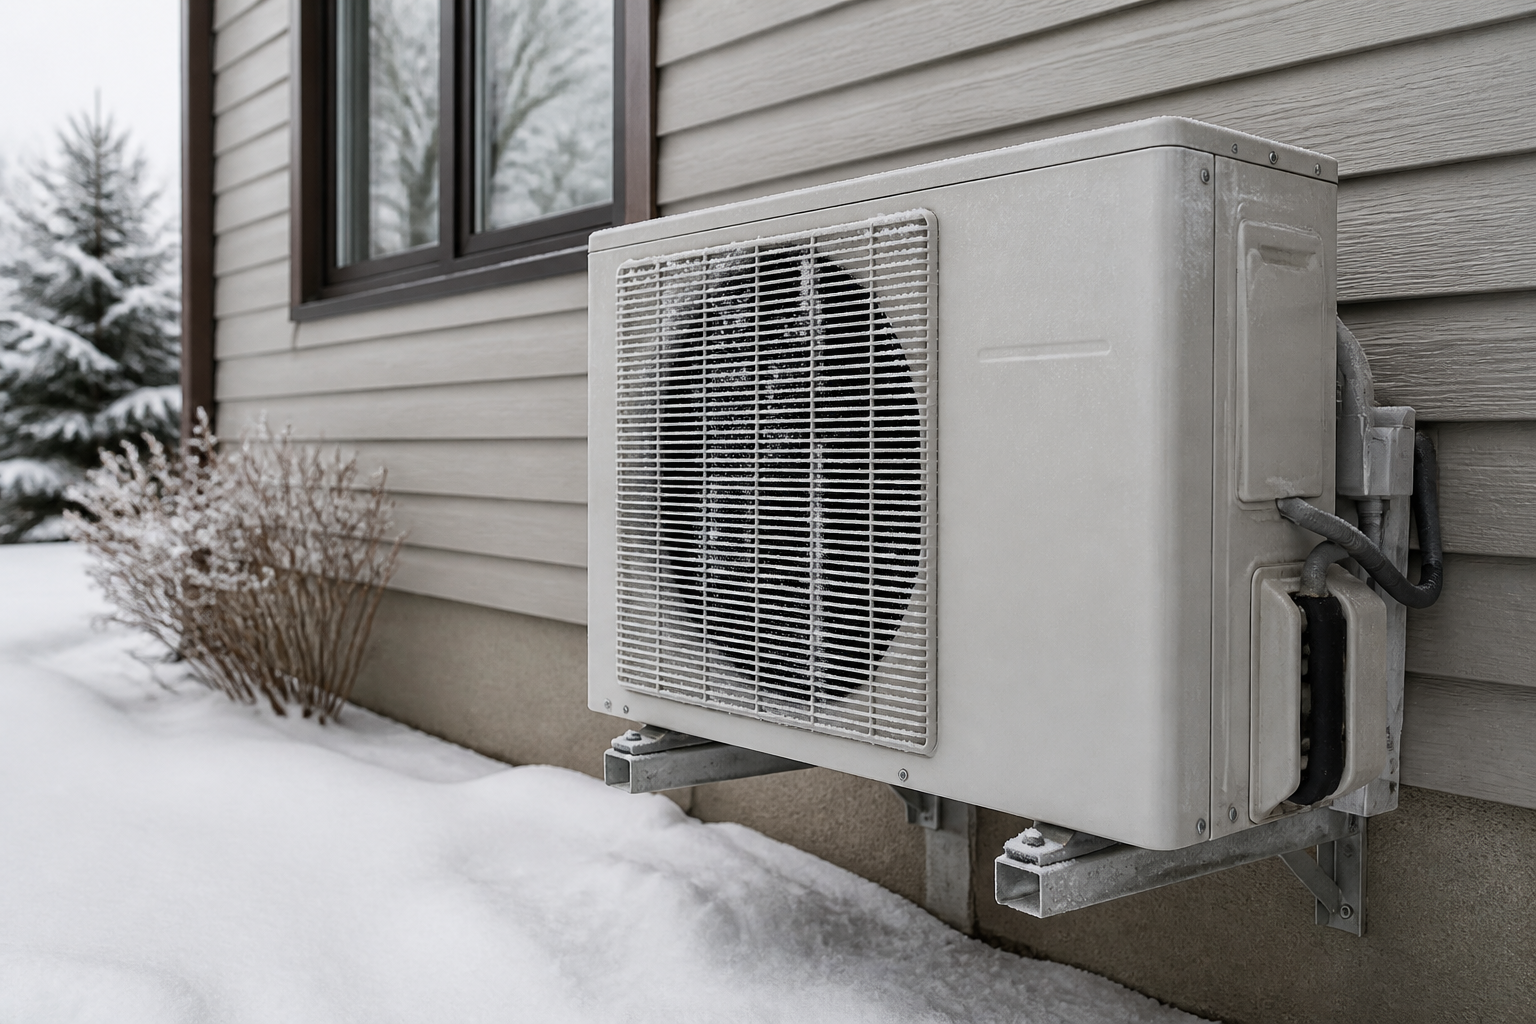
\includegraphics[width=0.58\linewidth]{images/book3/ai/b3-24-heat-pump-winter.png}

{\small An air-source \omterm{def:b1:heat-engines:machine}{heat pump} in winter: it takes heat from cold outdoor air and delivers three to four times the electrical energy it consumes to the house --- the weekend problem.}
\end{omfigure}

\section{Problem: The house heat pump}

\begin{problem}[{Weekend problem --- heating a house through a winter:
the bill with resistors, with gas, with an ideal heat pump and with a
real one, and where the real one's electricity goes}]
\label{pb:b1:heat-engines:1}
A house loses heat at the rate $K(T_{\mathrm{in}} - T_{\mathrm{out}})$ with
$K = \qty{250}{W/K}$; it is kept at $T_{\mathrm{in}} = \qty{20}{\degreeCelsius}$.
Design outdoor temperature $\qty{-5}{\degreeCelsius}$; heating season:
$200$ days with a mean outdoor temperature of \qty{7}{\degreeCelsius}.
Prices: electricity 0.25~\texteuro{} per \unit{kW h}, gas 0.10~\texteuro{} per
\unit{kW h}; $\qty{1}{kW h} = \qty{3.6}{MJ}$.

\medskip
\noindent\textbf{Part I --- The house and the old ways.}
\begin{enumerate}
  \item Heating power needed at the design temperature.
  \item Energy needed over the season, in joules and in \unit{kW h}.
  \item Cost of the season with electric \omterm{def:b1:dc-circuits:resistor}{resistors}.
  \item Cost with a gas boiler of \omterm{def:b1:heat-engines:efficiency}{efficiency} $0.90$.
  \item The electricity comes from a thermal power station of \omterm{def:b1:heat-engines:efficiency}{efficiency}
        $0.40$. Fuel energy consumed, per season, by the \omterm{def:b1:dc-circuits:resistor}{resistors} and by
        the boiler; comment on ``electric heating is thermodynamically
        wasteful''.
\end{enumerate}

\medskip
\noindent\textbf{Part II --- The ideal \omterm{def:b1:heat-engines:machine}{heat pump}.}
\begin{enumerate}[resume]
  \item Define $e_p$ and prove, from the two laws over one cycle, that
        $e_p \leq T_{\mathrm{in}}/(T_{\mathrm{in}} - T_{\mathrm{out}})$.
  \item Ideal $e_p$ at the design temperature, and the electrical power
        then needed.
  \item Ideal $e_p$ at the season's mean temperature, and (taking that
        value for the whole season) the seasonal electricity.
  \item Explain physically why $e_p$ falls when the outdoor temperature
        falls, and why this is the worst possible behaviour for a heating
        device.
  \item At the design point the ideal pump draws \qty{0.53}{kW} and
        delivers \qty{6.25}{kW}: where do the other \qty{5.7}{kW} come from,
        and why does cooling the cold outdoor air to heat a warm house
        not violate the second law?
\end{enumerate}

\medskip
\noindent\textbf{Part III --- The real machine.}
The pump runs a \omterm{def:b1:heat-engines:vapourcycle}{vapour-compression cycle}. The \omterm{def:b1:heat-engines:vapourcycle}{refrigerant} evaporates at
$T_{\mathrm{ev}} = T_{\mathrm{out}} - \qty{8}{K}$ and condenses at
$T_{\mathrm{cd}} = \qty{313}{K}$ (the water of a floor-heating circuit runs at
\qty{35}{\degreeCelsius}); the machine achieves $0.55$ of the Carnot
value computed between $T_{\mathrm{ev}}$ and $T_{\mathrm{cd}}$. Latent heat of
the \omterm{def:b1:heat-engines:vapourcycle}{refrigerant}: $L = \qty{200}{kJ/kg}$.
\begin{enumerate}[resume]
  \item Name the four components of the cycle, say in which the fluid
        receives $Q_c$, gives $|Q_h|$ and receives $W$, and why the
        evaporator must be colder than the outdoor air and the
        condenser hotter than the house.
  \item At the design temperature: $T_{\mathrm{ev}}$, and the Carnot $e_p$
        between $T_{\mathrm{ev}}$ and $T_{\mathrm{cd}}$.
  \item Real $e_p$, electrical power drawn, and heat taken from the
        outdoor air, at the design temperature.
  \item Mass flow rate of \omterm{def:b1:heat-engines:vapourcycle}{refrigerant} through the evaporator.
  \item Same questions (real $e_p$, electrical power) at the mean
        temperature of \qty{7}{\degreeCelsius}, where the house loses
        \qty{3.25}{kW}.
  \item Give $e_p$ as a function of $T_{\mathrm{out}}$; seasonal electricity
        and cost, taking the mean-temperature $e_p$ for the season.
        Compare with Part~I.
  \item Fuel energy consumed at the power station for the heat-pump
        season; compare with the \omterm{def:b1:dc-circuits:resistor}{resistors} and the boiler.
  \item A cold snap at \qty{-15}{\degreeCelsius}: heat demand, real $e_p$,
        electrical power if the pump could deliver it. The compressor's
        capacity actually falls with $T_{\mathrm{ev}}$ and the pump can only
        deliver \qty{3.8}{kW} there: backup \omterm{def:b1:dc-circuits:resistor}{resistor} power needed, and
        the meaning of ``sizing a \omterm{def:b1:heat-engines:machine}{heat pump}''.
  \item Had the house old radiators needing water at
        \qty{60}{\degreeCelsius} ($T_{\mathrm{cd}} = \qty{338}{K}$): real $e_p$
        and electrical power at the design temperature; conclude on the
        choice of emitters.
\end{enumerate}

\medskip
\noindent\textbf{Part IV --- Where the electricity goes.}
\begin{enumerate}[resume]
  \item Show that for a \omterm{def:b1:heat-engines:machine}{heat pump} delivering $|Q_h|$ to the house at
        $T_{\mathrm{in}}$ from outdoor air at $T_{\mathrm{out}}$,
        $W = |Q_h|(1 - T_{\mathrm{out}}/T_{\mathrm{in}}) + T_{\mathrm{out}}S_{\mathrm{created}}$.
  \item At the design point, entropy created per second by the heat
        transfer across the condenser (from \qty{313}{K} to the house) and
        across the evaporator (from the outdoor air to \qty{260}{K}).
  \item Electrical power these two temperature gaps cost; fraction of
        the \qty{1.92}{kW} drawn.
  \item Total entropy created per second by the real machine (compare
        its \qty{1.92}{kW} with the ideal \qty{0.53}{kW}); share of the
        exchangers; name the other sources.
  \item Halve the two gaps (\qty{4}{K} and \qty{10}{K}): entropy created
        in the exchangers and electrical power saved; what does halving
        a gap cost the designer?
  \item Sum up in three numbers: kilowatt-hours of heat per
        kilowatt-hour of electricity over the season; seasonal cost
        against gas; and, with electricity at \qty{60}{g} of CO$_2$ per
        \unit{kW h} and gas at \qty{200}{g}, the carbon emitted by each
        route.
\end{enumerate}
\end{problem}
